\documentclass[10pt]{article}
\usepackage[utf8]{inputenc}
\usepackage[T1]{fontenc}
\usepackage{graphicx}
\usepackage[export]{adjustbox}
\graphicspath{ {./images/} }
\usepackage{amsmath}
\usepackage{amsfonts}
\usepackage{amssymb}
\usepackage[version=4]{mhchem}
\usepackage{stmaryrd}

\title{Underfitting and Overfitting }


\author{Martin Jaggi\\
Last updated on: October 3, 2023}
\date{}


\begin{document}
\maketitle
Machine Learning Course - CS-433

credits to Mohammad Emtiyaz Khan \& Rüdiger Urbanke

EPFL

\section*{Motivation}
Models can be too limited or they can be too rich. In the first case we cannot find a function that is a good fit for the data in our model. We then say that we underfit. In the second case we have such a rich model family that we do not just fit the underlying function but we in fact fit the noise in the data as well. We then talk about an overfit. Both of these phenomena are undesirable. This discussion is made more difficult since all we have is data and so we do not know a priori what part is the underlying signal and what part is noise.

\section*{Underfitting with Linear Models}
It is easy to see that linear models might underfit. Consider a scalar case as shown in the figure below.

\begin{center}
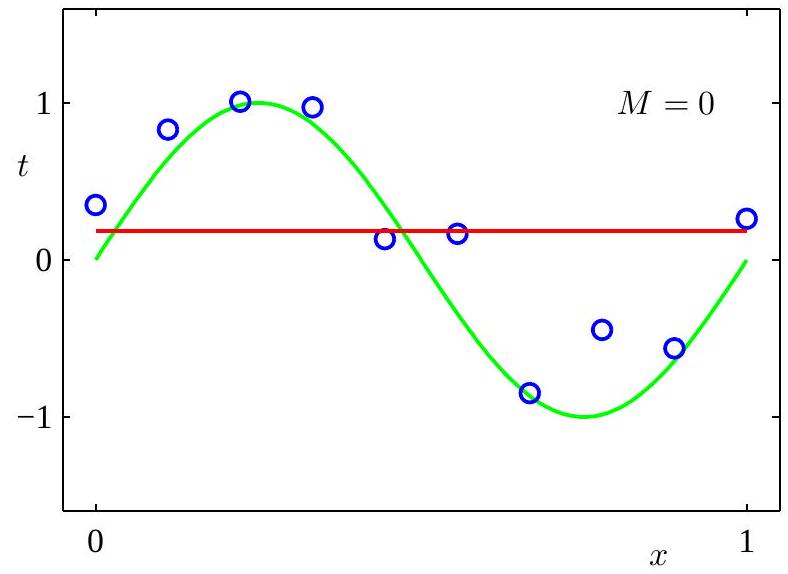
\includegraphics[max width=\textwidth]{2023_12_30_cfff7db3d8d5672f46efg-2}
\end{center}

The solid curve is the underlying function and the circles are the actual data. E.g., we assume that there is a scalar function $g(x)$ but that we do not observe $g\left(x_{n}\right)$ directly but only a noisy version of it, $y_{n}=g\left(x_{n}\right)+Z_{n}$, where $Z_{n}$ is
the noise. The noise might be due for example to some measurement inaccuracies. The $y_{n}$ are shown as blue cirles. If our model family consists of only linear functions of the scalar input $x$, i.e., $\mathcal{F}=\left\{f_{w}(x)=w x\right\}$, where $w$ is a scalar constant (the slope of the function), then it is clear that we cannot match the given function accurately, regardless how many samples we get and how small the noise is. We therefore will underfit.

Extended/Augmented Feature Vectors From the above example it might seem that linear models are too simple to ever overfit. But in fact, linear models are highly prone to overfitting, much more so than complicated models like neural nets.

Since linear models are inherently not very rich the following is a standard "trick" to make them more powerful.

In order to increase the representational power of linear models we typically "augment" the input. E.g., if the input (feature) is one-dimensional we might add a polynomial basis (of arbitrary degree $M$ ),

$$
\boldsymbol{\phi}\left(x_{n}\right):=\left[1, x_{n}, x_{n}^{2}, x_{n}^{3}, \ldots, x_{n}^{M}\right]
$$

so that we end up with an extended feature vector.

We then fit a linear model to this extended feature vector $\phi\left(x_{n}\right)$ :

$$
y_{n} \approx w_{0}+w_{1} x_{n}+w_{2} x_{n}^{2}+\ldots+w_{M} x_{n}^{M}=: \boldsymbol{\phi}\left(x_{n}\right)^{\top} \mathbf{w}
$$

\section*{Overfitting with Linear Models}
In the following four figures, circles are data points, the green line represents the "true function", and the red line is the model. The parameter $M$ is the maximum degree in the polynomial basis.
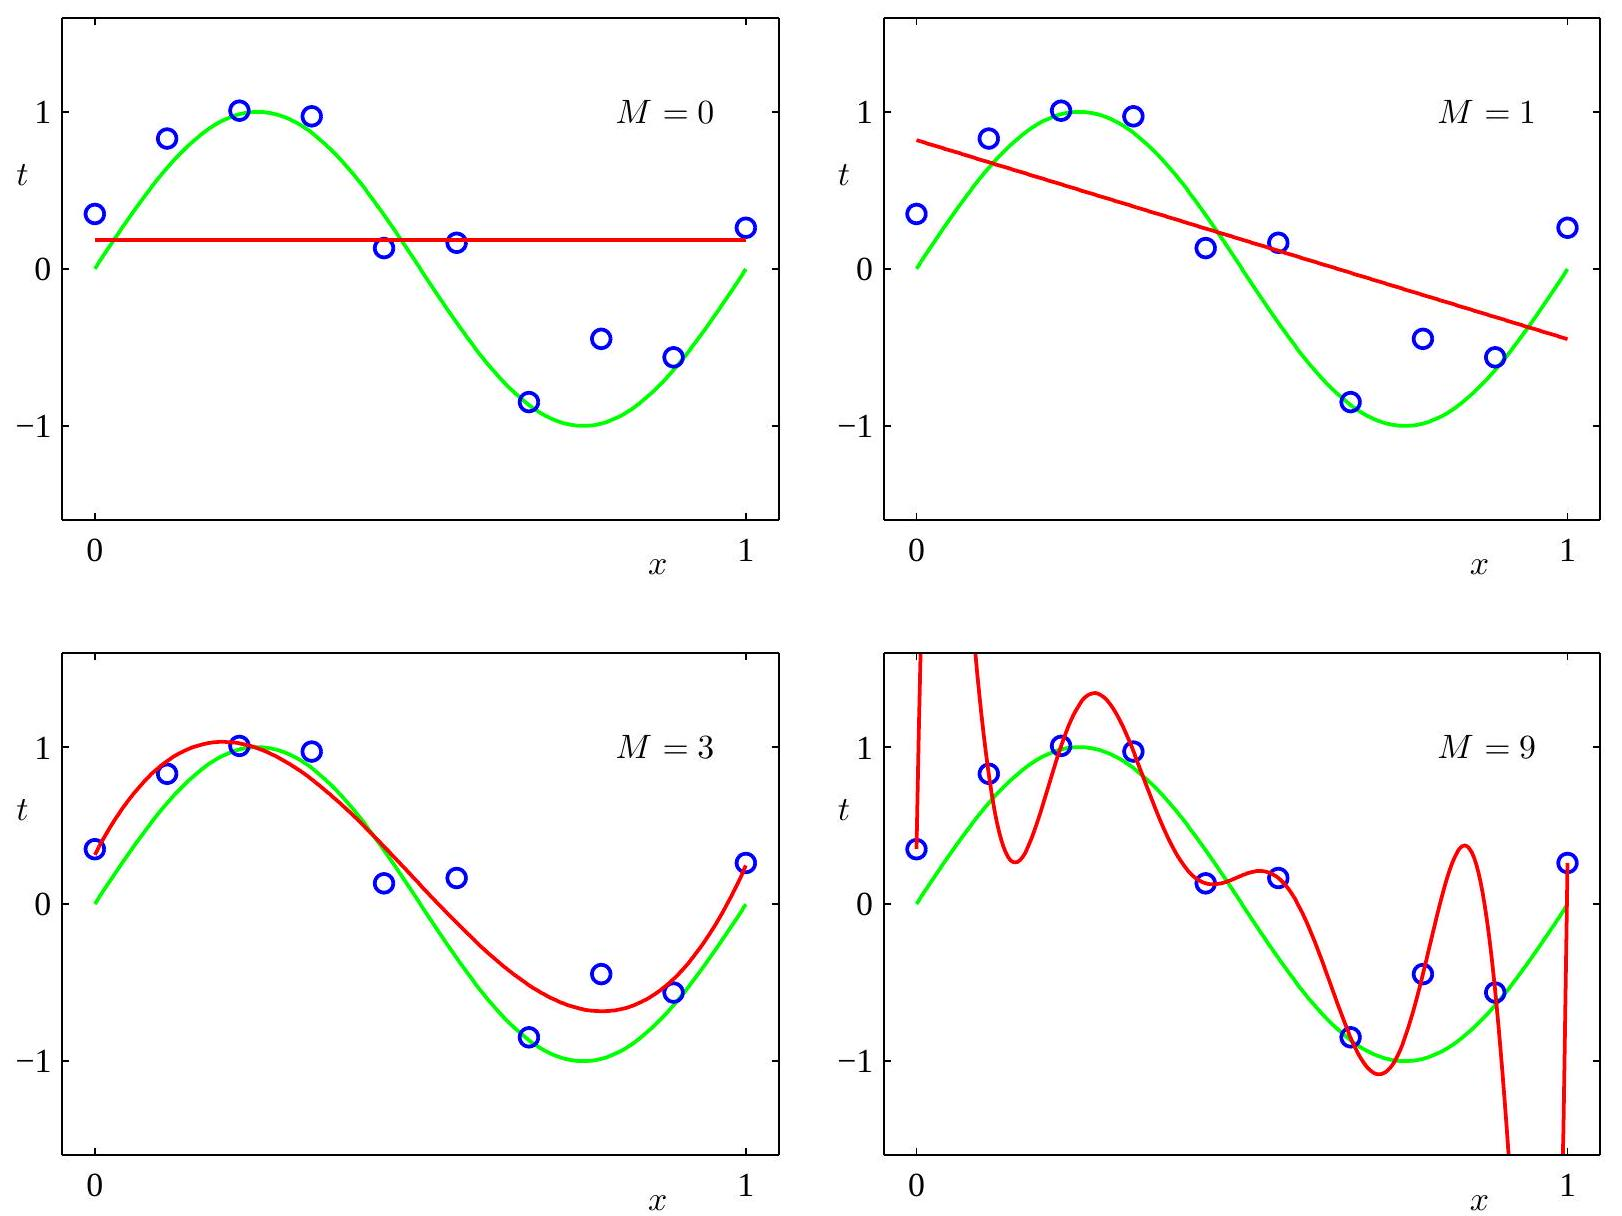
\includegraphics[max width=\textwidth, center]{2023_12_30_cfff7db3d8d5672f46efg-4}

For $M=0$ (the model is a constant) the model is underfitting and the same is true for $M=1$. For $M=3$ the model fits the data fairly well and is not yet so rich as to fit in addition the small "wiggles" caused by the noise. But for $M=9$ we now have such a rich model that it can fit every single data point and we see severe overfitting taking place. What can we do to avoid overfitting? If you increase the amount of data (increase $N$, but keep $M$ fixed), overfitting
might reduce. This is shown in the following two figures where we again consider the same model complexity $M=9$ but we have extra data $(N=15$ or even $N=100)$.
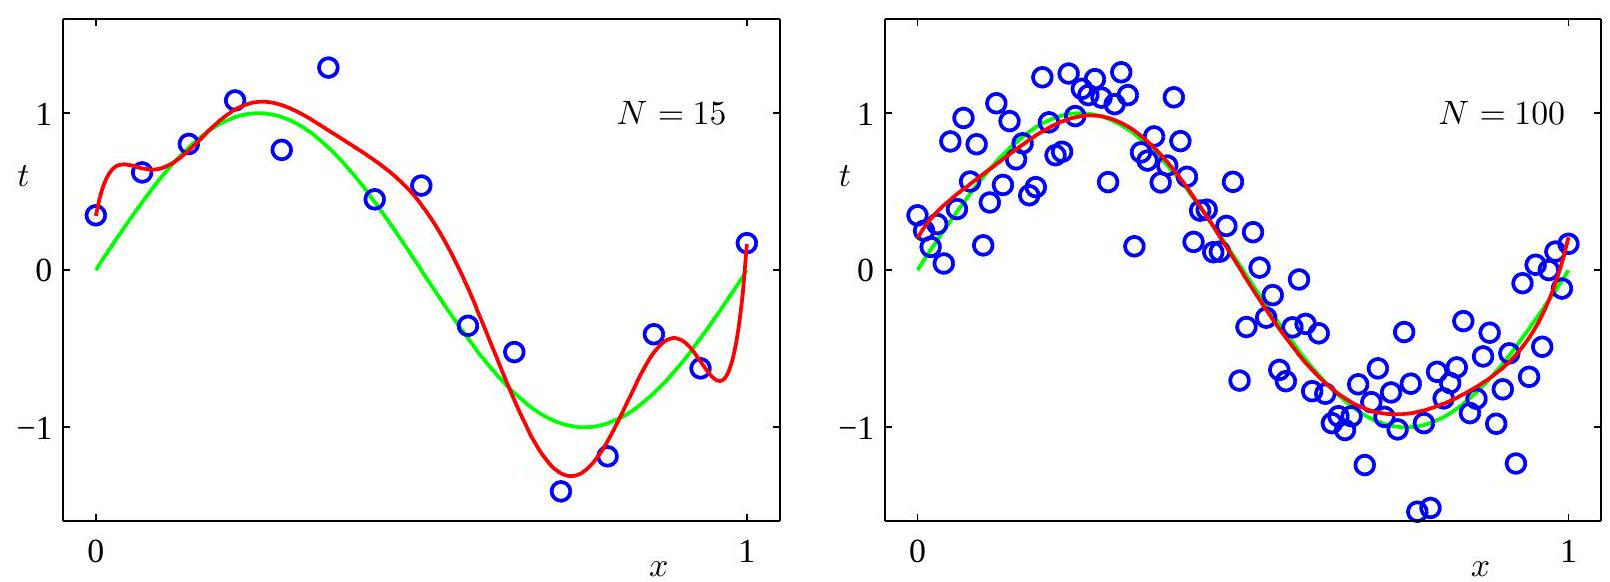
\includegraphics[max width=\textwidth, center]{2023_12_30_cfff7db3d8d5672f46efg-5}

\section*{A Word About Notation}
If it is important to distinguish the original input $\mathbf{x}$ from the augmented input then we will use $\phi(\mathbf{x})$ to denote this augmented input vector. But we can consider this augmentation as part of the pre-processing, and then we might simply write $\mathbf{x}$ to denote the input. This will save us a lot of notation.

\section*{Additional Materials}
Read about overfitting in the paper by Pedro Domingos (Sections 3 and 5 of "A few useful things to know about machine learning").


\end{document}